\documentclass[main.tex]{subfiles}

\begin{document}

\renewcommand{\labelitemi}{\ding{226}}
\renewcommand{\labelitemii}{\ding{227}}

\chapter{Super FGD}
\label{ch:up:sfgd}
A new scintillator target is going to be installed

\section{Conceptual design}

\begin{figure}[!ht]
	\centering
	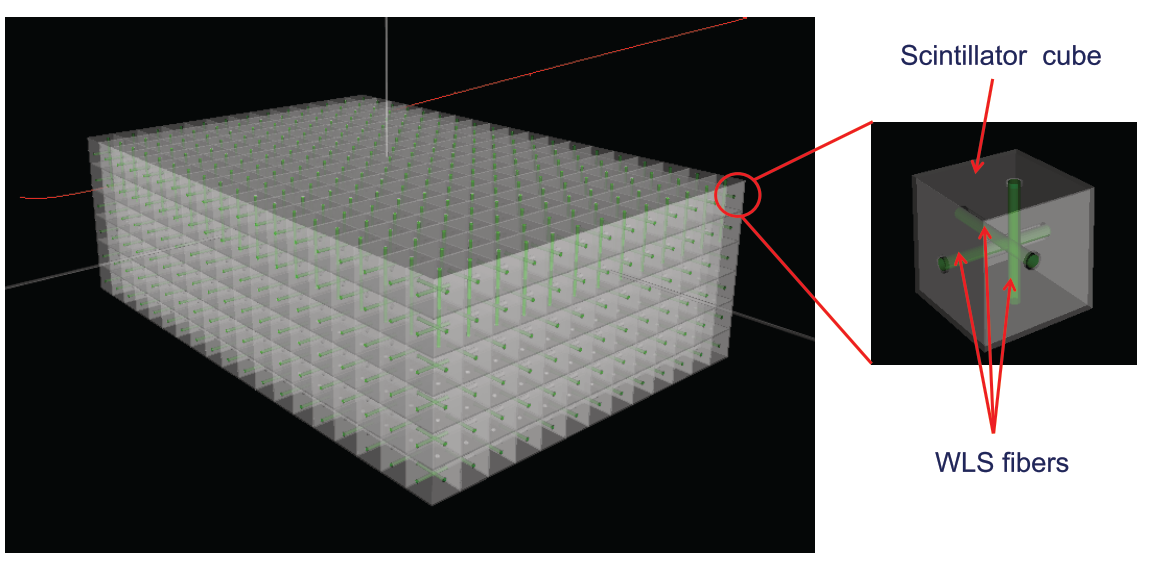
\includegraphics[width=0.8\linewidth]{sfgd_gen}
	\caption{The schematic concept of the SuperFGD detector made with scintillator cubes. Wavelength shifting fibers are used for the signal readout. The size of each cube is 1$\times$1$\times$1 $\text{cm}^3$.}
	\label{fig:up:sfgd:gen}
\end{figure}

\subsection{Assembly}

\section{Simulations}

\subsection{Expected light yield}

\subsection{Michell electron tagging}

\subsection{Pileups}






\section{Beamtest}

\subsection{First CERN beamtest}

\subsection{Second CERN beamtest}

\chapter{Neutron tagging in SuperFGD}
\label{ch:up:neutron}
\section{Motivation}
\section{Geant4 simulation}
\section{Efficiency and energy resolution}
\section{Background estimations}
\section{Prospects for physics}
\end{document}